% This is "sig-alternate.tex" V2.1 April 2013
% This file should be compiled with V2.5 of "sig-alternate.cls" May 2012
%
% This example file demonstrates the use of the 'sig-alternate.cls'
% V2.5 LaTeX2e document class file. It is for those submitting
% articles to ACM Conference Proceedings WHO DO NOT WISH TO
% STRICTLY ADHERE TO THE SIGS (PUBS-BOARD-ENDORSED) STYLE.
% The 'sig-alternate.cls' file will produce a similar-looking,
% albeit, 'tighter' paper resulting in, invariably, fewer pages.
%
% ----------------------------------------------------------------------------------------------------------------
% This .tex file (and associated .cls V2.5) produces:
%       1) The Permission Statement
%       2) The Conference (location) Info information
%       3) The Copyright Line with ACM data
%       4) NO page numbers
%
% as against the acm_proc_article-sp.cls file which
% DOES NOT produce 1) thru' 3) above.
%
% Using 'sig-alternate.cls' you have control, however, from within
% the source .tex file, over both the CopyrightYear
% (defaulted to 200X) and the ACM Copyright Data
% (defaulted to X-XXXXX-XX-X/XX/XX).
% e.g.
% \CopyrightYear{2007} will cause 2007 to appear in the copyright line.
% \crdata{0-12345-67-8/90/12} will cause 0-12345-67-8/90/12 to appear in the copyright line.
%
% ---------------------------------------------------------------------------------------------------------------
% This .tex source is an example which *does* use
% the .bib file (from which the .bbl file % is produced).
% REMEMBER HOWEVER: After having produced the .bbl file,
% and prior to final submission, you *NEED* to 'insert'
% your .bbl file into your source .tex file so as to provide
% ONE 'self-contained' source file.
%
% ================= IF YOU HAVE QUESTIONS =======================
% Questions regarding the SIGS styles, SIGS policies and
% procedures, Conferences etc. should be sent to
% Adrienne Griscti (griscti@acm.org)
%
% Technical questions _only_ to
% Gerald Murray (murray@hq.acm.org)
% ===============================================================
%
% For tracking purposes - this is V2.0 - May 2012
\documentclass{sig-alternate-05-2015}

\usepackage[hidelinks]{hyperref}
\usepackage{color}

\begin{document}

% Copyright
%\setcopyright{acmcopyright}
%\setcopyright{acmlicensed}
\setcopyright{rightsretained}
%\setcopyright{usgov}
%\setcopyright{usgovmixed}
%\setcopyright{cagov}
%\setcopyright{cagovmixed}


% DOI
\doi{}

% ISBN
\isbn{}

%Conference
\conferenceinfo{UCORE '16}{September 1st, Montreal, QC, Canada}

% \acmPrice{\$15.00}

%
% --- Author Metadata here ---
% \conferenceinfo{WOODSTOCK}{'97 El Paso, Texas USA}
%\CopyrightYear{2007} % Allows default copyright year (20XX) to be over-ridden - IF NEED BE.
%\crdata{0-12345-67-8/90/01}  % Allows default copyright data (0-89791-88-6/97/05) to be over-ridden - IF NEED BE.
% --- End of Author Metadata ---

\title{Centre of Pressure Capture \& Reconstruction in Physically-Based Character Animation}

\subtitle{[12th Undergraduate Computer Science Research Symposium]}

%
% You need the command \numberofauthors to handle the 'placement
% and alignment' of the authors beneath the title.
%
% For aesthetic reasons, we recommend 'three authors at a time'
% i.e. three 'name/affiliation blocks' be placed beneath the title.
%
% NOTE: You are NOT restricted in how many 'rows' of
% "name/affiliations" may appear. We just ask that you restrict
% the number of 'columns' to three.
%
% Because of the available 'opening page real-estate'
% we ask you to refrain from putting more than six authors
% (two rows with three columns) beneath the article title.
% More than six makes the first-page appear very cluttered indeed.
%
% Use the \alignauthor commands to handle the names
% and affiliations for an 'aesthetic maximum' of six authors.
% Add names, affiliations, addresses for
% the seventh etc. author(s) as the argument for the
% \additionalauthors command.
% These 'additional authors' will be output/set for you
% without further effort on your part as the last section in
% the body of your article BEFORE References or any Appendices.

\numberofauthors{2} %  in this sample file, there are a *total*
% of EIGHT authors. SIX appear on the 'first-page' (for formatting
% reasons) and the remaining two appear in the \additionalauthors section.
%
\author{
% You can go ahead and credit any number of authors here,
% e.g. one 'row of three' or two rows (consisting of one row of three
% and a second row of one, two or three).
%
% The command \alignauthor (no curly braces needed) should
% precede each author name, affiliation/snail-mail address and
% e-mail address. Additionally, tag each line of
% affiliation/address with \affaddr, and tag the
% e-mail address with \email.
%
% 1st. author
\alignauthor
Monty Thibault \\
	   \affaddr{Undergraduate Researcher}\\
	   \affaddr{Mathematics \& Computer Science, McGill}\\
       \email{monty.thibault@mail.mcgill.ca}
% 2nd. author
\alignauthor
Paul Kry\\
       \affaddr{Associate Professor}\\
       \affaddr{McGill School of Computer Science}\\
       \email{kry@cs.mcgill.ca}
% 3rd. author
}
% There's nothing stopping you putting the seventh, eighth, etc.
% author on the opening page (as the 'third row') but we ask,
% for aesthetic reasons that you place these 'additional authors'
% in the \additional authors block, viz.

% Just remember to make sure that the TOTAL number of authors
% is the number that will appear on the first page PLUS the
% number that will appear in the \additionalauthors section.

\maketitle

\begin{figure}
\noindent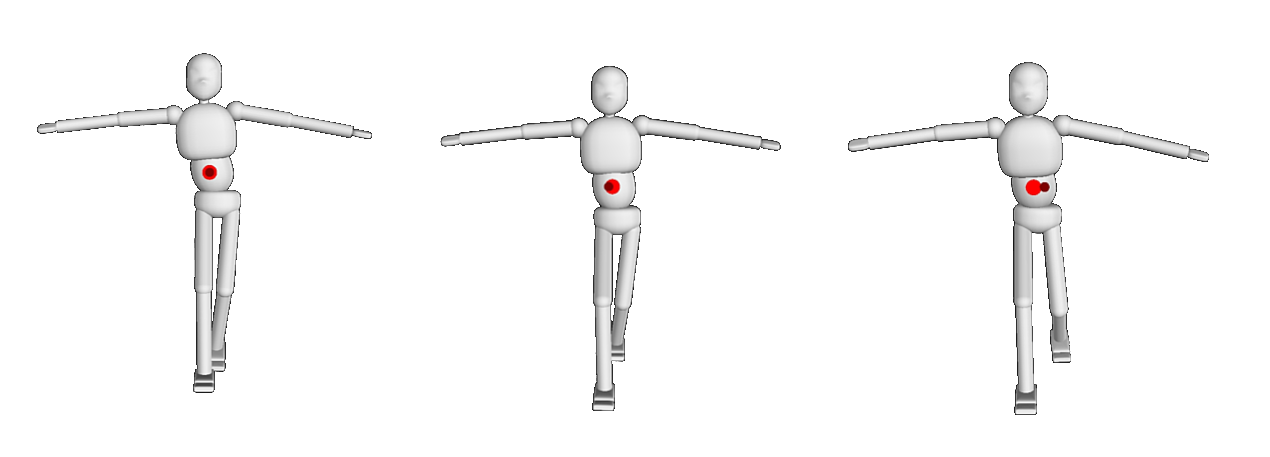
\includegraphics[width=250pt]{snip_fig}
\caption{Virtual characters in mid-stride. The red dots signify their centres of mass. \href{https://youtu.be/JGDUO0vYXK0}{\color{blue} See the video.}}
\label{fig:cartwheel}
\end{figure}

\begin{abstract}
	
	Over the past two decades, research on controlling balance in virtual characters has largely focused on the problems of achieving robust standing balance and that of robust locomotion. Balance controllers have been developed around a variety of principles, including linear momentum control\cite{Macchietto:2009:MCB:1531326.1531386}, angular momentum control\cite{Azad2016}, model-predictive control\cite{Wieber2006}, and virtual model control\cite{PrattDilworth1997}. They vary greatly in the assumptions about the nature of the balance or movement tasks, the abstractions used, and their reactive or anticipative nature. However, almost all balance algorithms presume that the center of mass and its velocity are known quantities that can be used within the control equations. This unfortunately allows virtual characters to potentially have super human balancing abilities. Previous work has demonstrated that natural and interesting degradation of a balance controller can be produced by injecting noise into the balance controller's gravity direction, or likewise by directly perturbing the control torques. 
	
	In this project, we have instead configured a force sensor apparatus (Figure 2) and captured data with the goal of building a model for the error that humans make in controlling their center of mass via the force they exert on the ground. The apparatus consists of four six-axis force sensors bolted to wooden boards. A participant is able to stand on the boards, with one sensor under the toe and heel of each foot.
	
	A software system solves for the centre of pressure from the torques and forces of all four sensors. A recording system captures samples at 100 Hz in a variety of poses, which is later used as the training set for an autoregressive-moving-average (ARMA) model. The fitted model can then be used to reconstruct the signal in the context of a real-time graphics engine (Figure 3). As part of the project, we have incorporated our technique into the existing, opensource animation software \emph{Cartwheel 3d}\cite{2010-TOG-gbwc} (Figure 1).

	Our system interfaces with the animation controller by modifying the percieved centre of \emph{mass} with our model of the centre of \emph{pressure}, plus some variable scaling coefficient. We have found this to be a reasonable approximation without sacrificing realism in the controller output.
	\begin{figure}[h!]
		\begin{center}
		\noindent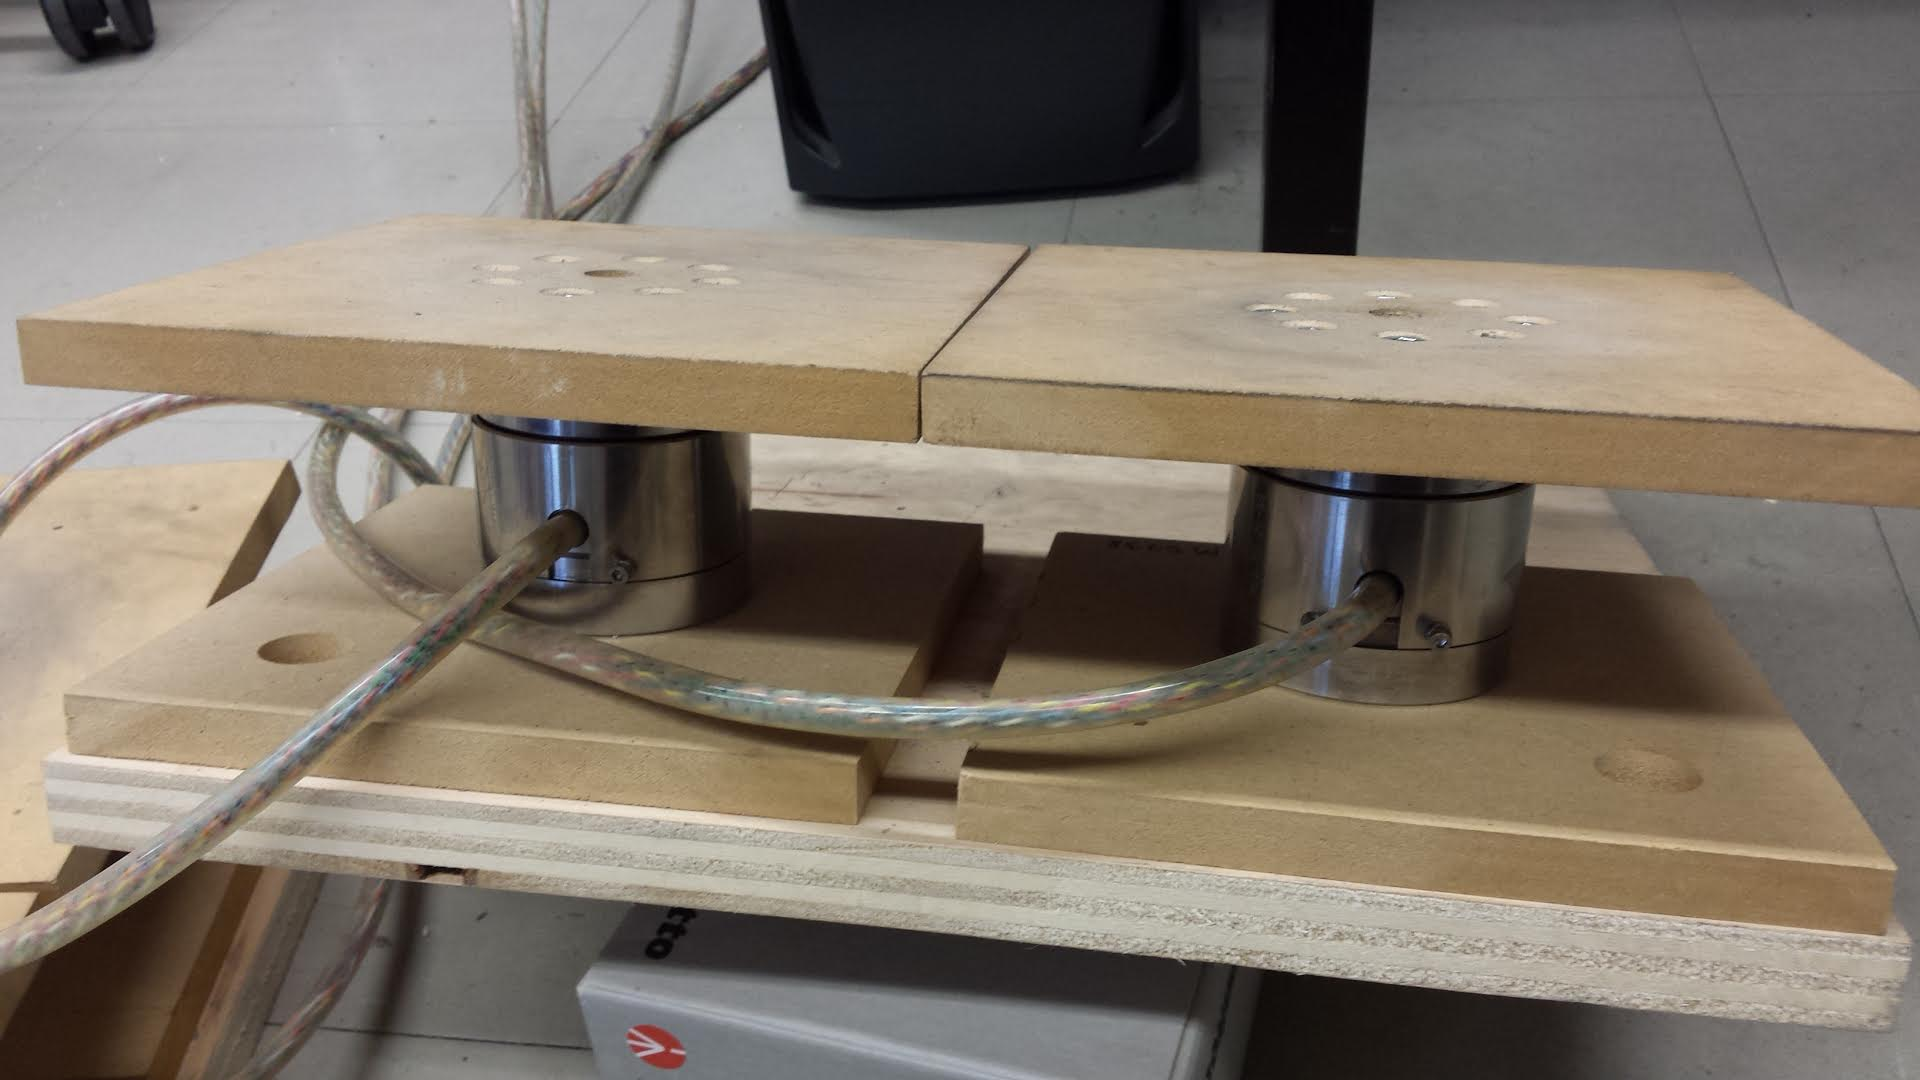
\includegraphics[width=225pt]{sensors_side}
		\noindent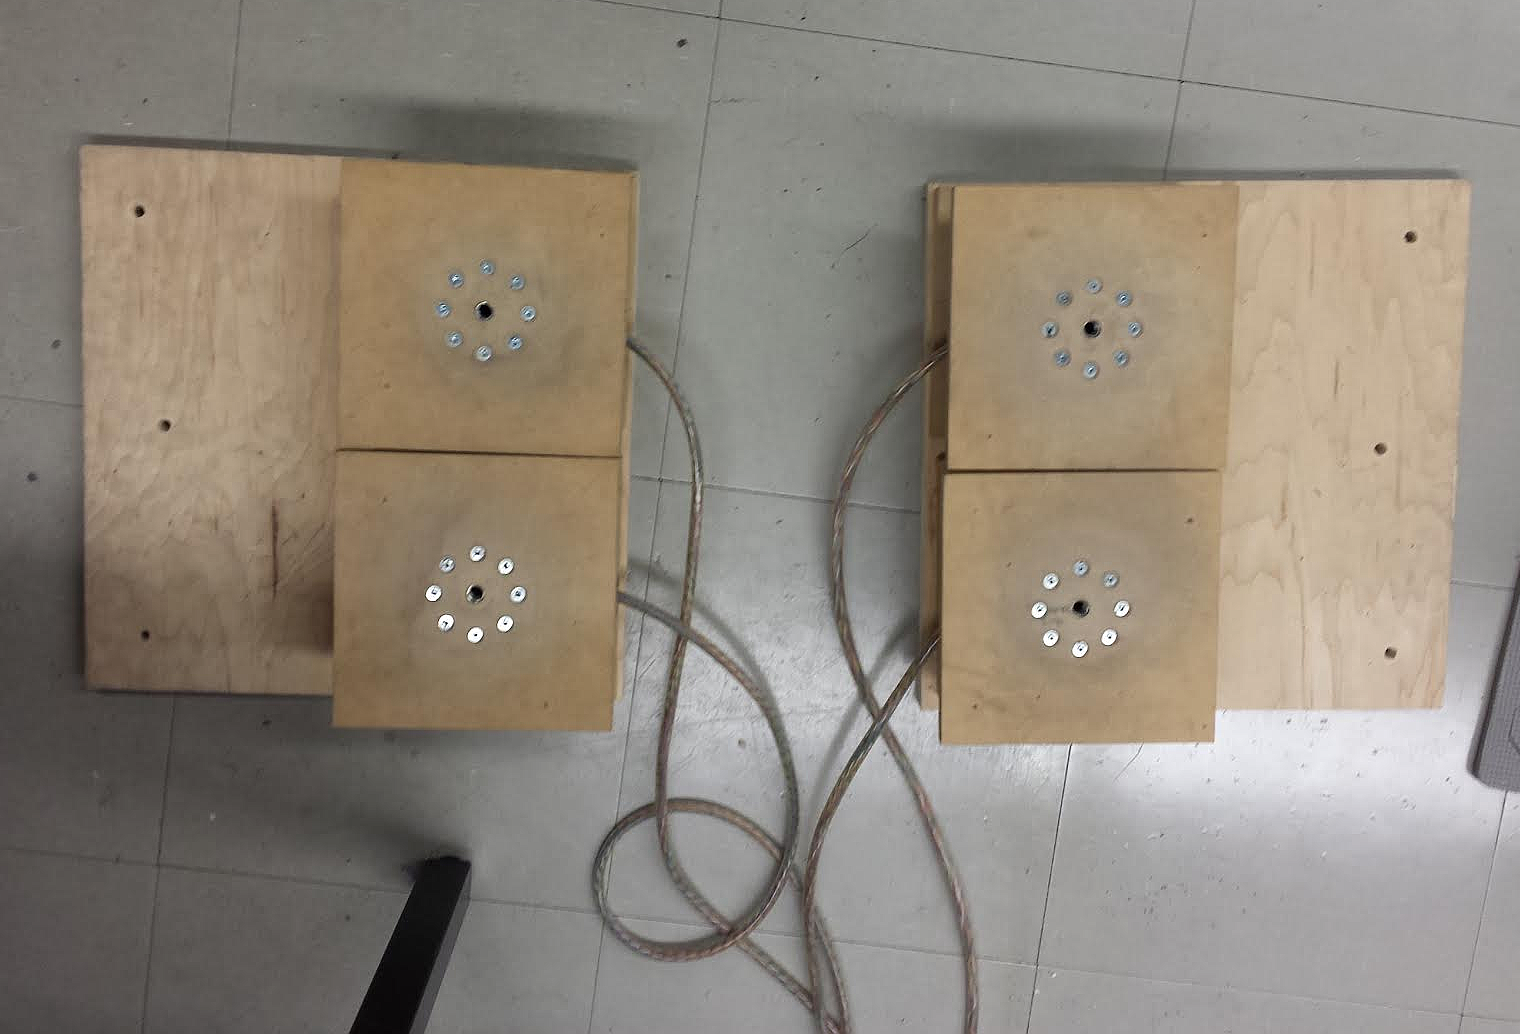
\includegraphics[width=225pt]{sensors_top}
		\caption{The force sensor apparatus}
	
		\end{center}
	\end{figure}
	
	\begin{figure*}
		\noindent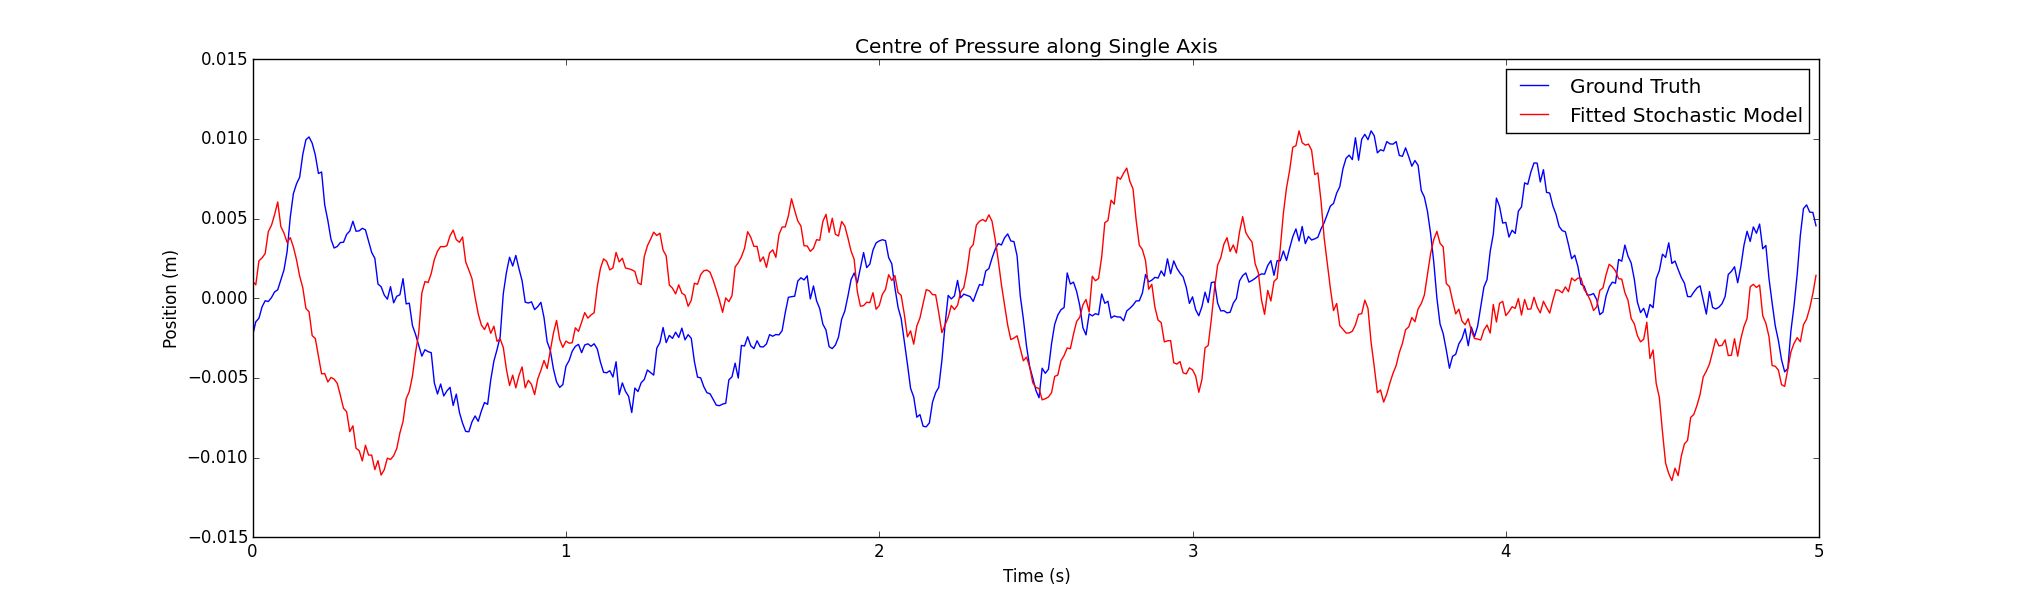
\includegraphics[width=\textwidth]{stochastic_model}
		\caption{Samples from (blue) a one-foot-balancing training set and (red) the associated ARMA model.}
		
	\end{figure*}
	
	The benefit of our appoach over a simple injection of white noise is that it can be powerfully generalized to incorporate exogenous variables: such examples include but are not limited to controller states and environmental factors that affect centre of balance. Such a system could allow one to develop a probabilistic approximation of character error to use alongside, for instance, motion-capture data. This is a possible route for future work in this area.
	
	Our work finds application in any media involving animation. Video games and virtual reality are particularly relevant, as a physically-based animation approach merits user interaction and autonomy; moreover, realistic human locomotion in these domains have been rarely achieved, in part due to unrealistic assumptions that our research addresses.
	
\end{abstract}

\bibliographystyle{unsrt}
\bibliography{sigproc}


\iffalse

\section{Conclusions}
This paragraph will end the body of this sample document.
Remember that you might still have Acknowledgments or
Appendices; brief samples of these
follow.  There is still the Bibliography to deal with; and
we will make a disclaimer about that here: with the exception
of the reference to the \LaTeX\ book, the citations in
this paper are to articles which have nothing to
do with the present subject and are used as
examples only.
%\end{document}  % This is where a 'short' article might terminate

%ACKNOWLEDGMENTS are optional
\section{Acknowledgments}
This section is optional; it is a location for you
to acknowledge grants, funding, editing assistance and
what have you.  In the present case, for example, the
authors would like to thank Gerald Murray of ACM for
his help in codifying this \textit{Author's Guide}
and the \textbf{.cls} and \textbf{.tex} files that it describes.

%
% The following two commands are all you need in the
% initial runs of your .tex file to
% produce the bibliography for the citations in your paper.
\bibliographystyle{abbrv}
\bibliography{sigproc}  % sigproc.bib is the name of the Bibliography in this case
% You must have a proper ".bib" file
%  and remember to run:
% latex bibtex latex latex
% to resolve all references
%
% ACM needs 'a single self-contained file'!
%
%APPENDICES are optional
%\balancecolumns
\appendix
%Appendix A
\section{Headings in Appendices}
The rules about hierarchical headings discussed above for
the body of the article are different in the appendices.
In the \textbf{appendix} environment, the command
\textbf{section} is used to
indicate the start of each Appendix, with alphabetic order
designation (i.e. the first is A, the second B, etc.) and
a title (if you include one).  So, if you need
hierarchical structure
\textit{within} an Appendix, start with \textbf{subsection} as the
highest level. Here is an outline of the body of this
document in Appendix-appropriate form:
\subsection{Introduction}
\subsection{The Body of the Paper}
\subsubsection{Type Changes and  Special Characters}
\subsubsection{Math Equations}
\paragraph{Inline (In-text) Equations}
\paragraph{Display Equations}
\subsubsection{Citations}
\subsubsection{Tables}
\subsubsection{Figures}
\subsubsection{Theorem-like Constructs}
\subsubsection*{A Caveat for the \TeX\ Expert}
\subsection{Conclusions}
\subsection{Acknowledgments}
\subsection{Additional Authors}
This section is inserted by \LaTeX; you do not insert it.
You just add the names and information in the
\texttt{{\char'134}additionalauthors} command at the start
of the document.
\subsection{References}
Generated by bibtex from your ~.bib file.  Run latex,
then bibtex, then latex twice (to resolve references)
to create the ~.bbl file.  Insert that ~.bbl file into
the .tex source file and comment out
the command \texttt{{\char'134}thebibliography}.
% This next section command marks the start of
% Appendix B, and does not continue the present hierarchy
\section{More Help for the Hardy}
The sig-alternate.cls file itself is chock-full of succinct
and helpful comments.  If you consider yourself a moderately
experienced to expert user of \LaTeX, you may find reading
it useful but please remember not to change it.
%\balancecolumns % GM June 2007
% That's all folks!

\fi

\end{document}
